\documentclass[12pt, psamsfonts]{amsart}

%-------Packages---------
\usepackage{amssymb,amsfonts}
\usepackage[all,arc]{xy}
\usepackage{enumerate}
\usepackage{mathrsfs}
\usepackage{theoremref}
\usepackage{graphicx}
\usepackage[bookmarks]{hyperref}

%--------Theorem Environments--------
%theoremstyle{plain} --- default
\newtheorem{thm}{Theorem}[section]
\newtheorem{cor}[thm]{Corollary}
\newtheorem{prop}[thm]{Proposition}
\newtheorem{lem}[thm]{Lemma}
\newtheorem{conj}[thm]{Conjecture}
\newtheorem{quest}[thm]{Question}

\theoremstyle{definition}
\newtheorem{defn}[thm]{Definition}
\newtheorem{defns}[thm]{Definitions}
\newtheorem{con}[thm]{Construction}
\newtheorem{exmp}[thm]{Example}
\newtheorem{exmps}[thm]{Examples}
\newtheorem{notn}[thm]{Notation}
\newtheorem{notns}[thm]{Notations}
\newtheorem{addm}[thm]{Addendum}
\newtheorem{exer}[thm]{Exercise}

\theoremstyle{remark}
\newtheorem{rem}[thm]{Remark}
\newtheorem{rems}[thm]{Remarks}
\newtheorem{warn}[thm]{Warning}
\newtheorem{sch}[thm]{Scholium}

\DeclareMathOperator{\Hom}{Hom}
\DeclareMathOperator{\Id}{Id}

\makeatletter
\let\c@equation\c@thm
\makeatother
\numberwithin{equation}{section}

\bibliographystyle{plain}

\begin{document}

\title{Math 601 Homework (Due 8/30)}
\author{Hidenori Shinohara}
\maketitle

\begin{exer}
  Show that a bijective ring homomorphism is an isomorphism in the category of rings.
\end{exer}

\begin{proof}
Let $f$ be a bijective ring homomorphism from a ring $A$ to a ring $B$.

Let $\mathbf{C}$ denote the category of rings.
Then $A, B$ are objects of the category $\mathbf{C}$.
Since $\Hom_{\mathbf{C}}(A, B)$ is defined to be the set of all ring homomorphisms from $A$ to $B$, $f \in \Hom_{\mathbf{C}}(A, B)$.

We will show that there exists an element $g \in \Hom_{\mathbf{C}}(B, A)$ such that $g \circ f = \Id_A$ and $f \circ g = \Id_B$.

Let a function $g: B \rightarrow A$ be defined such that $\forall b \in B, g(b) = a$ where $a$ is an element such that $f(a) = b$.
$g$ is well-defined because:

\begin{itemize}
  \item
    $f$ is surjective, so there exists an $a \in A$ such that $f(a) = b$.
  \item
    $f$ is injective, so such an $a$ must be unique.
\end{itemize}

We claim that this $g$ satisfies the desired properties:

\begin{itemize}
  \item
    Claim 1: $g \in \Hom_{\mathbf{C}}(B, A)$.
    This is equivalent to showing that $g$ is a ring homomorphism.
    Let $b_1, b_2 \in B$ be given.
    Let $a_1 = g(b_1), a_2 = g(b_2)$.
    Then $f(a_1) = b_1$ and $f(a_2) = b_2$.
    \begin{itemize}
      \item
        Since $f$ is a ring homomorphism, $f(a_1 + a_2) = f(a_1) + f(a_2) = b_1 + b_2$.
        Therefore, $g(b_1 + b_2) = a_1 + a_2 = g(b_1) + g(b_2)$.
      \item
        Since $f$ is a ring homomorphism, $f(a_1 \cdot a_2) = f(a_1) \cdot f(a_2) = b_1 \cdot b_2$.
        Therefore, $g(b_1 \cdot b_2) = a_1 \cdot a_2 = g(b_1) \cdot g(b_2)$.
      \item
        Since $f$ is a ring homomorphism, $f(1) = 1$.
        Thus $g(1) = 1$.
    \end{itemize}
    Therefore, $g \in \Hom_{\mathbf{C}}(B, A)$.
  \item
    Claim 2: $ g \circ f = \Id_A$.
    Let $a \in A$.
    Let $b = f(a)$.
    Then $g(b) = a$, so $g(f(a)) = a$.
    This implies that $\forall a \in A, g(f(a)) = a$.
    Thus $g \circ f = \Id_A$.
  \item
    Claim 3: $ f \circ g = \Id_B$.
    Let $b \in B$.
    Let $a = g(b)$.
    Then $f(a) = b$, so $f(g(b)) = b$.
    Therefore, $\forall b \in B, f(g(b)) = b$.
    Thus $f \circ g = \Id_B$.
\end{itemize}

Therefore, $f$ is indeed an isomorphism in the category of rings.
\end{proof}

\begin{exer}
  Let $A$ and $B$ be two objects in a category $\mathbf{C}$.
  An object, $P$, of $\mathbf{C}$ together with two morphisms, $p_A \in \Hom_{\mathbf{C}}(P, A), p_B \in \Hom_{\mathbf{C}}(P, B)$, is a product of $A$ and $B$ if the following property holds:
  Given any object $C$ of $\mathbf{C}$ and any two morphisms, $f \in \Hom_{\mathbf{C}}(C, A)$ and $g \in \Hom_{\mathbf{C}}(C, B)$, then there is a unique element, $h \in \Hom_{\mathbf{C}}(C, P)$ such that $f = p_A \circ h$ and $g = p_B \circ h$.
\end{exer}

\begin{proof}
  \begin{figure}
    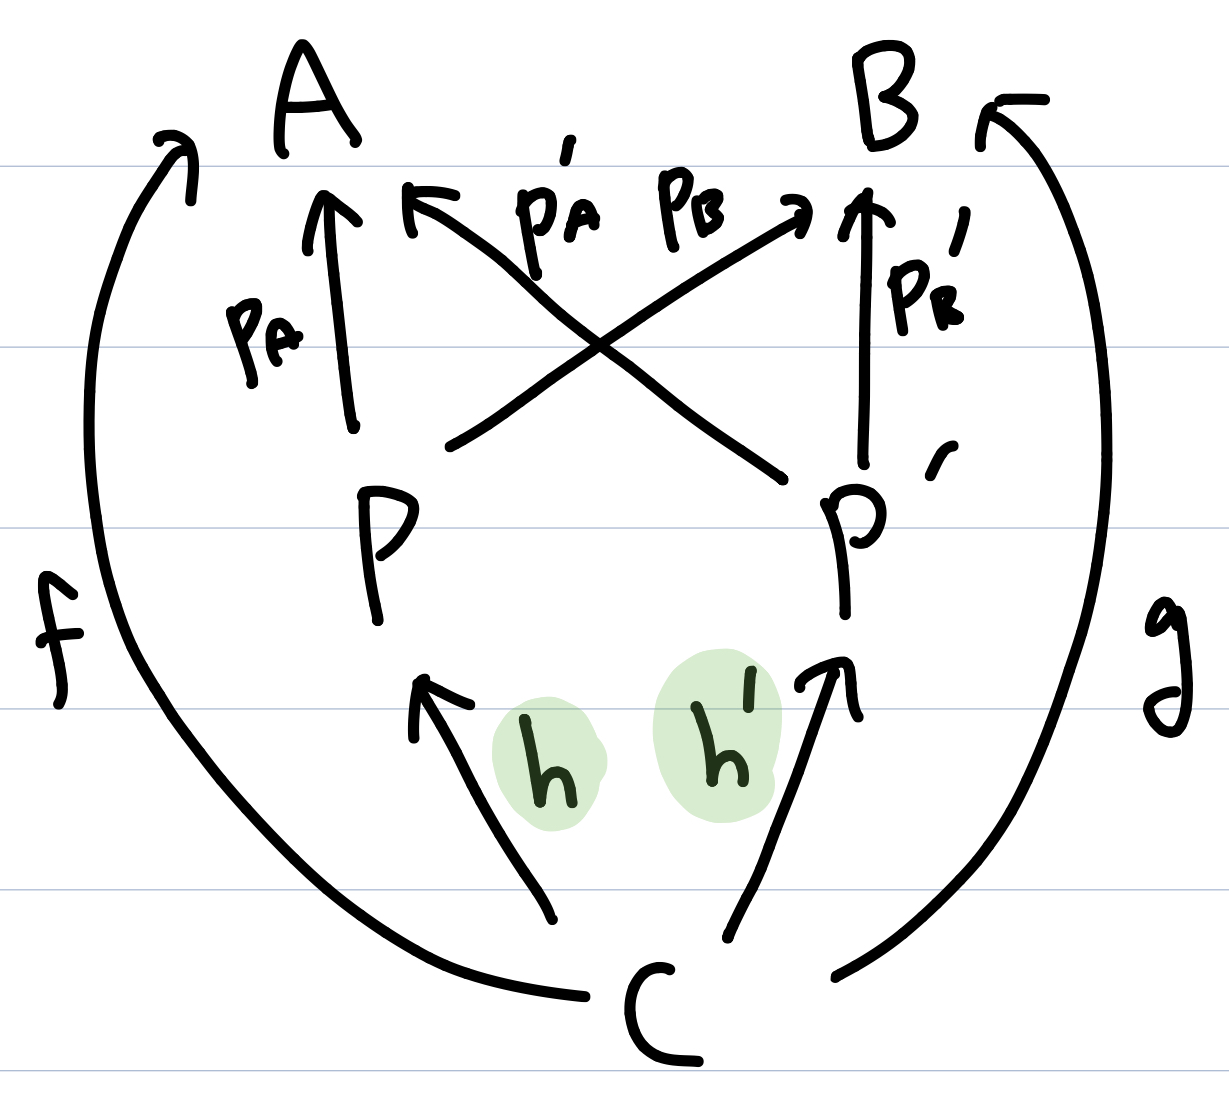
\includegraphics[width=\linewidth]{maps.jpeg}
      \caption{Diagram of maps for the second problem}
    \label{fig:maps}
  \end{figure}

  First, we will consider the case when $C = P, f = p_A, g = p_B$.

  Then there exists a unique map $h' \in \Hom_{\mathbf{C}}(C, P') = \Hom_{\mathbf{C}}(P, P')$ such that $f = p_A' \circ h'$.
  In other words, $p_A = p_A' \circ h'$.

  Similarly, we will consider the case when $C = P', f = p_A', g = p_B'$.
  Then there exists a unique map $h \in \Hom_{\mathbf{C}}(C, P) = \Hom_{\mathbf{C}}(P', P)$ such that $f = p_A \circ h$.
  In other words, $p_A' = p_A \circ h$.

  \begin{align*}
    p_A
      &= p_A' \circ h' \\
      &= (p_A \circ h) \circ h' \\
      &= p_A \circ (h \circ h')
  \end{align*}

  and 

  \begin{align*}
    p_A'
      &= p_A \circ h \\
      &= (p_A' \circ h') \circ h \\
      &= p_A' \circ (h' \circ h).
  \end{align*}

  Again, we will consider the case when $C = P, f = p_A, g = p_B$.
  Then there must exist a unique map $h'' \in \Hom_{\mathbf{C}}(P, P)$ such that $p_A = p_A \circ h''$.

  \begin{itemize}
    \item
      $p_A = p_A \circ (h \circ h')$.
    \item
      $p_A = p_A \circ \Id_P$.
  \end{itemize}

  Therefore, $h \circ h' = \Id_P$ because of the uniqueness of $h''$.

  Similarly, we will again consider the case when $C = P', f = p_A', g = p_B'$.
  Then there must exist a unique map $h''' \in \Hom_{\mathbf{C}}(P', P')$ such that $p_A' = p_A' \circ h'''$.

  \begin{itemize}
    \item
      $p_A' = p_A' \circ (h' \circ h)$.
    \item
      $p_A' = p_A' \circ \Id_{P'}$.
  \end{itemize}

  Therefore, $h' \circ h = \Id_{P'}$ because of the uniqueness of $h'''$.

  We showed that $h \in \Hom_{\mathbf{C}}(P', P)$ and $h' \in \Hom_{\mathbf{C}}(P, P')$ satisfy $h \circ h' = \Id_P$ and $h' \circ h = \Id_{P'}$.
  In addition, we showed that $p_A = p_A' \circ h'$ and $p_B = p_B' \circ h'$.
  Therefore, $h'$ is the desired isomorphism.
\end{proof}

\end{document}
